\documentclass[../../main.tex]{subfiles}
\graphicspath{{../../image/}{../../figure/}}
\begin{document}

\section{解的局部结构}\label{section:ch12-解的局部结构}

在本章中，$U$ 表示一个局部有界变差函数，定义在 $(-\infty,\infty)\times[0,\infty)$ 上，取值于以原点为中心、半径很小的圆盘内，它是系统\eqref{align:ch12-系统}的弱解，并在原书第 10.1 节所述意义下满足 Lax $E$-条件。
特别地，对任意凸熵--熵流对 $(\eta,q)$（其中 $\eta$ 为凸），
\begin{align}
\partial_t\eta(U(x,t))+\partial_x q(U(x,t))\leqslant 0
\label{align:ch12-熵不等式}
\end{align}
在测度意义下成立。

在第 X 章中发展的广义特征线概念，将在讨论中起关键作用。

\begin{definition}[类空曲线]\label{definition:ch12-类空曲线}
一条 Lipschitz 曲线，其图像 $\mathscr{A}$ 嵌入上半平面，称为相对于 $U$ 是类空的，如果对每一点 $(\bar x,\bar t)\in\mathscr{A}$ 成立下述性质：由从 $(\bar x,\bar t)$ 发出的极大后向 2-特征线 $\zeta(\cdot)$ 的图像与极小后向 1-特征线 $\xi(\cdot)$ 的图像之间所夹的点集 $\{(x,t):0\leqslant t<\bar t,\ \zeta(t)<x<\xi(t)\}$，与 $\mathscr{A}$ 的交集为空。
\end{definition}

显然，与 $U$ 相联系的任一族的广义特征线，都相对于 $U$ 是类空的。类似地，所有时间线 $t=$ 常数都是类空的。

解 $U$ 将通过其诱导的 Riemann 不变量坐标 $(z,w)$ 来方便地监测。在\cref{section:ch12-解的界}中将证明，沿类空曲线的 $z$ 与 $w$ 的迹的总变差由其初始数据的总变差控制。
预期这一结果，从今往后我们假设：对任意类空曲线 $t=t^*(x)$，$z(x\pm,t^*(x))$ 与 $w(x\pm,t^*(x))$ 都是有界变差函数，其总变差由某正常数 $\theta$ 界定。由于解的振幅很小且所有论证都是局部的，我们可不失一般性地设 $\theta$ 很小。

为描述解的局部结构，我们与上半平面的一般点 $(\bar x,\bar t)$ 相联系八条（不必互异的）曲线（见\cref{figure:ch12-八曲线}），其确定方式如下：

对 $t<\bar t$：$\xi_-(\cdot)$ 与 $\xi_+(\cdot)$ 是从 $(\bar x,\bar t)$ 发出的极小与极大后向 1-特征线；类似地，$\zeta_-(\cdot)$ 与 $\zeta_+(\cdot)$ 是从 $(\bar x,\bar t)$ 发出的极小与极大后向 2-特征线。

对 $t>\bar t$：$\varphi_+(\cdot)$ 是从 $(\bar x,\bar t)$ 发出的极大前向 1-特征线，$\psi_-(\cdot)$ 是极小前向 2-特征线。为确定其余两条曲线 $\varphi_-(\cdot)$ 与 $\psi_+(\cdot)$，我们考虑从一般点 $(x,t)$ 发出的极小后向 1-特征线 $\xi(\cdot)$ 与极大后向 2-特征线 $\zeta(\cdot)$，并定位这些特征线被 $\bar t$ 时间线所截的点 $\xi(\bar t)$ 与 $\zeta(\bar t)$。于是 $\varphi_-(t)$ 由下述性质确定：当 $x<\varphi_-(t)$ 时 $\xi(\bar t)<\bar x$，当 $x>\varphi_-(t)$ 时 $\xi(\bar t)\geqslant\bar x$。类似地，$\psi_+(t)$ 由下述性质刻画：当 $x<\psi_+(t)$ 时 $\zeta(\bar t)\leqslant\bar x$，当 $x>\psi_+(t)$ 时 $\zeta(\bar t)>\bar x$。特别地，$\varphi_-(t)\leqslant\varphi_+(t)$，且若 $\varphi_-(t)<x<\varphi_+(t)$ 则 $\xi(\bar t)=\bar x$。类似地，推得 $\psi_-(t)\leqslant\psi_+(t)$，且 $\psi_-(t)<x<\psi_+(t)$ 蕴含 $\zeta(\bar t)=\bar x$。

\begin{figure}[ht]
\centering
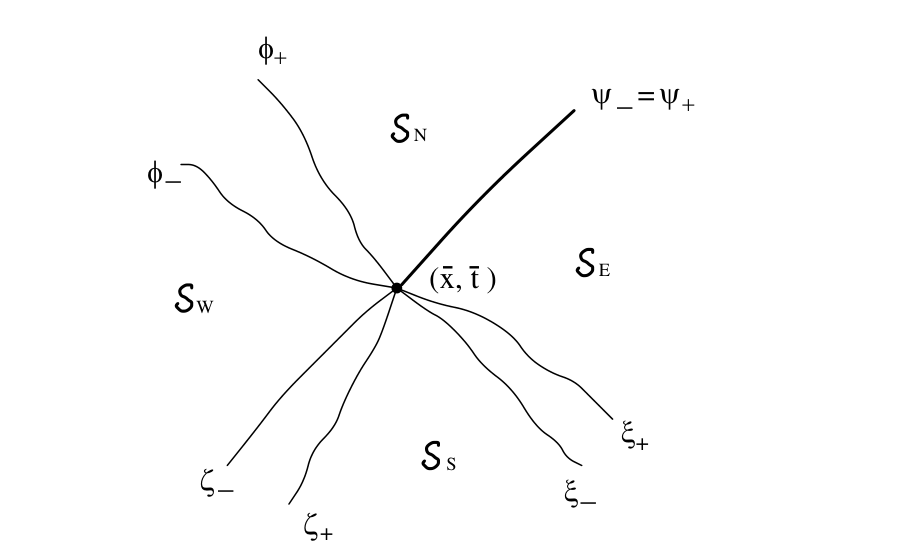
\includegraphics[width=0.75\textwidth]{ch12-fig03-01.png}
\caption{从 $(\bar x,\bar t)$ 发出的八条特征线与四个区域 $\mathscr{S}_W,\mathscr{S}_E,\mathscr{S}_N,\mathscr{S}_S$}
\label{figure:ch12-八曲线}
\end{figure}

固定 $\tau>\bar t$，令 $\xi_\tau(\cdot)$ 表示从点 $(\varphi_-(\tau),\tau)$ 发出的极小后向 1-特征线。再任取一序列 $\{x_m\}$ 从上方收敛于 $\varphi_-(\tau)$，令 $\xi_m(\cdot)$ 表示从 $(x_m,\tau)$ 发出的极小后向 1-特征线。于是序列 $\{\xi_m(\cdot)\}$ 或其子列，将收敛于某条从 $(\varphi_-(\tau),\tau)$ 发出的后向 1-特征线 $\hat\xi_\tau(\cdot)$。进而，对任意 $\bar t\leqslant t\leqslant\tau$，有 $\xi_\tau(t)\leqslant\varphi_-(t)\leqslant\xi_\tau(t)$。特别地，这蕴含 $\varphi_-(\cdot)$ 是一条 Lipschitz 连续的类空曲线，其斜率在 $\lambda$ 的取值范围内。类似地，$\psi_+(\cdot)$ 是一条 Lipschitz 连续的类空曲线，其斜率在 $\mu$ 的取值范围内。

再参见\cref{figure:ch12-八曲线}，我们看到上述曲线围成区域：
\begin{align}
\mathscr{S}_W&=\{(x,t):x<\bar x,\ \zeta_-^{-1}(x)<t<\varphi_-^{-1}(x)\},
\label{align:ch12-区域W}\\
\mathscr{S}_E&=\{(x,t):x>\bar x,\ \xi_+^{-1}(x)<t<\psi_+^{-1}(x)\},
\label{align:ch12-区域E}\\
\mathscr{S}_N&=\{(x,t):t>\bar t,\ \varphi_+(t)<x<\psi_-(t)\},
\label{align:ch12-区域N}\\
\mathscr{S}_S&=\{(x,t):t<\bar t,\ \zeta_+(t)<x<\xi_-(t)\}.
\label{align:ch12-区域S}
\end{align}

\begin{definition}[局部正则]\label{definition:ch12-局部正则}
称解在上半平面的点 $(\bar x,\bar t)$ 处\textbf{局部正则}，如果下述条件成立：
\begin{enumerate}[(a)]
\item\label{item:ch12-局部正则-a} 当 $(x,t)$ 穿过区域 $\mathscr{S}_W,\mathscr{S}_E,\mathscr{S}_N$ 或 $\mathscr{S}_S$ 中任一个趋于 $(\bar x,\bar t)$ 时，$(z(x\pm,t),w(x\pm,t))$ 分别趋于极限 $(z_W,w_W),(z_E,w_E),(z_N,w_N)$ 或 $(z_S,w_S)$，其中特别有 $z_W=z(\bar x-,\bar t)$、$w_W=w(\bar x-,\bar t)$、$z_E=z(\bar x+,\bar t)$、$w_E=w(\bar x+,\bar t)$。
\item\label{item:ch12-局部正则-b1} 若 $p_\ell(\cdot)$ 与 $p_r(\cdot)$ 是任意两条从 $(\bar x,\bar t)$ 发出的后向 1-特征线，且对 $t<\bar t$ 有 $\xi_-(t)\leqslant p_\ell(t)<p_r(t)\leqslant\xi_+(t)$，则
\begin{align}
z_S&=\lim_{t\uparrow\bar t}z(\xi_-(t)\pm,t)\leqslant\lim_{t\uparrow\bar t}z(p_\ell(t)-,t)\leqslant\lim_{t\uparrow\bar t}z(p_\ell(t)+,t)\nonumber\\
&\leqslant\lim_{t\uparrow\bar t}z(p_r(t)-,t)\leqslant\lim_{t\uparrow\bar t}z(p_r(t)+,t)\leqslant\lim_{t\uparrow\bar t}z(\xi_+(t)\pm,t)=z_E,
\label{align:ch12-正则1z}\\
w_S&=\lim_{t\uparrow\bar t}w(\xi_-(t)\pm,t)\geqslant\lim_{t\uparrow\bar t}w(p_\ell(t)-,t)\geqslant\lim_{t\uparrow\bar t}w(p_\ell(t)+,t)\nonumber\\
&\geqslant\lim_{t\uparrow\bar t}w(p_r(t)-,t)\geqslant\lim_{t\uparrow\bar t}w(p_r(t)+,t)\geqslant\lim_{t\uparrow\bar t}w(\xi_+(t)\pm,t)=w_E.
\label{align:ch12-正则1w}
\end{align}
\item\label{item:ch12-局部正则-b2} 若 $q_\ell(\cdot)$ 与 $q_r(\cdot)$ 是任意两条从 $(\bar x,\bar t)$ 发出的后向 2-特征线，且对 $t<\bar t$ 有 $\zeta_-(t)\leqslant q_\ell(t)<q_r(t)\leqslant\zeta_+(t)$，则
\begin{align}
w_W&=\lim_{t\uparrow\bar t}w(\zeta_-(t)\pm,t)\geqslant\lim_{t\uparrow\bar t}w(q_\ell(t)-,t)\geqslant\lim_{t\uparrow\bar t}w(q_\ell(t)+,t)\nonumber\\
&\geqslant\lim_{t\uparrow\bar t}w(q_r(t)-,t)\geqslant\lim_{t\uparrow\bar t}w(q_r(t)+,t)\geqslant\lim_{t\uparrow\bar t}w(\zeta_+(t)\pm,t)=w_S,
\label{align:ch12-正则2w}\\
z_W&=\lim_{t\uparrow\bar t}z(\zeta_-(t)\pm,t)\leqslant\lim_{t\uparrow\bar t}z(q_\ell(t)-,t)\leqslant\lim_{t\uparrow\bar t}z(q_\ell(t)+,t)\nonumber\\
&\leqslant\lim_{t\uparrow\bar t}z(q_r(t)-,t)\leqslant\lim_{t\uparrow\bar t}z(q_r(t)+,t)\leqslant\lim_{t\uparrow\bar t}z(\zeta_+(t)\pm,t)=z_S.
\label{align:ch12-正则2z}
\end{align}
\item\label{item:ch12-局部正则-c1} 若对 $\bar t<t<\bar t+s$ 有 $\varphi_-(t)=\varphi_+(t)$，则 $z_W\leqslant z_N$、$w_W\geqslant w_N$。另一方面，若对 $\bar t<t<\bar t+s$ 有 $\varphi_-(t)<\varphi_+(t)$，则 $w_W=w_N$，且当 $(x,t)$ 穿过区域 $\{(x,t):t>\bar t,\ \varphi_-(t)<x<\varphi_+(t)\}$ 趋于 $(\bar x,\bar t)$ 时，$w(x\pm,t)$ 趋于 $w_W$。进而，若 $p_\ell(\cdot)$ 与 $p_r(\cdot)$ 是任意两条从 $(\bar x,\bar t)$ 发出的前向 1-特征线，且对 $\bar t<t<\bar t+s$ 有 $\varphi_-(t)\leqslant p_\ell(t)\leqslant p_r(t)\leqslant\varphi_+(t)$，则
\begin{align}
z_W&=\lim_{t\downarrow\bar t}z(\varphi_-(t)\pm,t)\geqslant\lim_{t\downarrow\bar t}z(p_\ell(t)-,t)=\lim_{t\downarrow\bar t}z(p_\ell(t)+,t)\nonumber\\
&\geqslant\lim_{t\downarrow\bar t}z(p_r(t)-,t)=\lim_{t\downarrow\bar t}z(p_r(t)+,t)\geqslant\lim_{t\downarrow\bar t}z(\varphi_+(t)\pm,t)=z_N.
\label{align:ch12-正则3z}
\end{align}
\item\label{item:ch12-局部正则-c2} 若对 $\bar t<t<\bar t+s$ 有 $\psi_-(t)=\psi_+(t)$，则 $w_N\geqslant w_E$、$z_N\leqslant z_E$。另一方面，若对 $\bar t<t<\bar t+s$ 有 $\psi_-(t)<\psi_+(t)$，则 $z_N=z_E$，且当 $(x,t)$ 穿过区域 $\{(x,t):t>\bar t,\ \psi_-(t)<x<\psi_+(t)\}$ 趋于 $(\bar x,\bar t)$ 时，$z(x\pm,t)$ 趋于 $z_E$。进而，若 $q_\ell(\cdot)$ 与 $q_r(\cdot)$ 是任意两条从 $(\bar x,\bar t)$ 发出的前向 2-特征线，且对 $\bar t<t<\bar t+s$ 有 $\psi_-(t)\leqslant q_\ell(t)\leqslant q_r(t)\leqslant\psi_+(t)$，则
\begin{align}
w_N&=\lim_{t\downarrow\bar t}w(\psi_-(t)\pm,t)\leqslant\lim_{t\downarrow\bar t}w(q_\ell(t)-,t)=\lim_{t\downarrow\bar t}w(q_\ell(t)+,t)\nonumber\\
&\leqslant\lim_{t\downarrow\bar t}w(q_r(t)-,t)=\lim_{t\downarrow\bar t}w(q_r(t)+,t)\leqslant\lim_{t\downarrow\bar t}w(\psi_+(t)\pm,t)=w_E.
\label{align:ch12-正则4w}
\end{align}
\end{enumerate}
\end{definition}

上述定义的动机在于

\begin{theorem}\label{theorem:ch12-局部正则存在}
当 $\theta$ 充分小时，解在上半平面的任一点处局部正则。
\end{theorem}

证明将在下一节给出。然而，此处应先作如下说明。定义\cref{definition:ch12-局部正则}的动机来源于分段光滑解的经验。事实上，在局部正则点，两个特征族的入射波碰撞产生跳跃间断，随后该间断被分解为出射波扇。陈述\ref{item:ch12-局部正则-b1}与\ref{item:ch12-局部正则-b2}调控入射波，允许可容许激波与聚焦压缩波的任意组合。陈述\ref{item:ch12-局部正则-c1}与\ref{item:ch12-局部正则-c2}刻画出射波扇。特别地，\ref{item:ch12-局部正则-c1}蕴含左状态 $(z_W,w_W)$ 可与右状态 $(z_N,w_N)$ 由一个 1-稀疏波或可容许 1-激波连接；而\ref{item:ch12-局部正则-c2}蕴含左状态 $(z_N,w_N)$ 可与右状态 $(z_E,w_E)$ 由一个 2-稀疏波或可容许 2-激波连接。因此，出射波扇由以 $(z(\bar x-,\bar t),w(\bar x-,\bar t))$ 与 $(z(\bar x+,\bar t),w(\bar x+,\bar t))$ 为左右状态的 Riemann 问题解局部逼近。

\cref{theorem:ch12-局部正则存在}的一个简单推论是：$\varphi_-(\cdot)$ 是一条 1-特征线，而 $\psi_+(\cdot)$ 是一条 2-特征线。

定义\cref{definition:ch12-局部正则}与\cref{theorem:ch12-局部正则存在}甚至适用于初始线 $\bar t=0$ 上的点，只要删去陈述中关于 $t<\bar t$ 的无关部分。然而应注意，$\bar t=0$ 与 $\bar t>0$ 之间存在重要差别。在前一情形，$(z(\bar x\pm,0),w(\bar x\pm,0))$ 不受约束，可由初始数据任意给定，因而出射波扇可包含激波与稀疏波的任意组合。相比之下，当 $\bar t>0$ 时，定义\cref{definition:ch12-局部正则}中的\ref{item:ch12-局部正则-b1}与\ref{item:ch12-局部正则-b2}诱导出限制 $z_W\leqslant z_E$ 与 $w_W\geqslant w_E$。这与\ref{item:ch12-局部正则-c1}、\ref{item:ch12-局部正则-c2}结合，排除了两个出射波均为稀疏波的可能。

\end{document}
